
%(BEGIN_QUESTION)
% Copyright 2006, Tony R. Kuphaldt, released under the Creative Commons Attribution License (v 1.0)
% This means you may do almost anything with this work of mine, so long as you give me proper credit

Studer følgende pH-målekrets, og svar på spørsmålene:

$$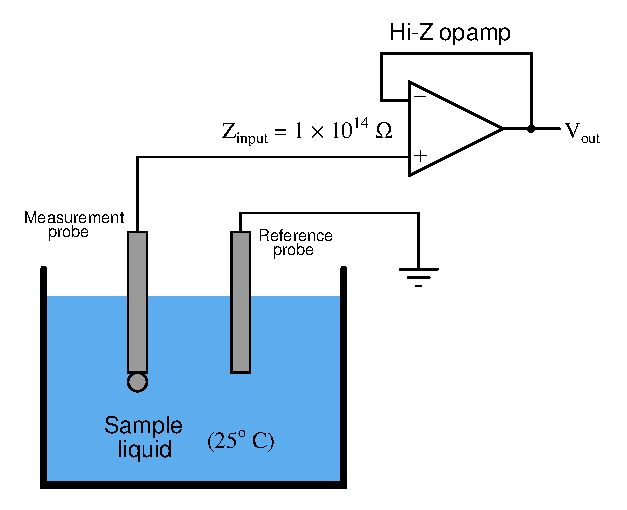
\includegraphics[width=15.5cm]{i00925x01.eps}$$

\begin{itemize}
\item{} Beregn ideell utgangsspenning fra de to pH-probene hvis løsningens hydrogenion-konsentrasjon er 0.0065 M.  $V_{probe}$ = \underbar{\hskip 50pt} volt
\vskip 5pt
\item{} Vil utgangsspenningen {\it øke}, {\it minke}, eller {\it være uendret} sammenlignet med det du nettopp beregnet hvis en svært liten mengde sur substans tilsettes væsken?
\vskip 5pt
\item{} Vil utgangsspenningen {\it øke}, {\it minke}, eller {\it være uendret} hvis motstanden i måleproben øker kraftig på grunn av belegg?
\vskip 5pt
\item{} Beregn faktisk utgangsspenning fra op-ampen hvis måleelektrodens motstand er 9.5 $\times$ 10$^{12}$ ohm og probene genererer 130 mV. Anta at referanseprobens motstand er lav nok til å neglisjeres.  $V_{output}$ = \underbar{\hskip 50pt} volt
\end{itemize}

\vfil 

\underbar{file i00925}
\eject
%(END_QUESTION)





%(BEGIN_ANSWER)

Dette er en vurderingsoppgave -- ingen fasit eller hint oppgis!

%(END_ANSWER)





%(BEGIN_NOTES)

\begin{itemize}
\item{} Beregn ideell utgangsspenning fra de to pH-probene hvis løsningens hydrogenion-konsentrasjon er 0.0065 M.  $V_{probe}$ = \underbar{\bf 284.7 mV}
\vskip 5pt
\item{} Utgangsspenningen vil {\bf øke} hvis en svært liten mengde sur substans tilsettes væsken.
\vskip 5pt
\item{} Utgangsspenningen vil {\bf minke} litt hvis motstanden i måleproben øker kraftig på grunn av belegg. Svaret {\bf være uendret} godtas også, fordi reduksjonen normalt er svært liten.
\vskip 5pt
\item{} $V_{output}$ = \underbar{\bf 118.72 mV}
\end{itemize}

%INDEX% Chemistry, pH: Nernst voltage and slope calculations

%(END_NOTES)

